\documentclass[conference]{IEEEtran}
\IEEEoverridecommandlockouts
% The preceding line is only needed to identify funding in the first footnote. If that is unneeded, please comment it out.
\usepackage{cite}
\usepackage{amsmath,amssymb,amsfonts}
\usepackage{algorithmic}
\usepackage{graphicx}
\usepackage{placeins}
\usepackage{textcomp}
\usepackage{xcolor}
\usepackage{hyperref}
\def\BibTeX{{\rm B\kern-.05em{\sc i\kern-.025em b}\kern-.08em
    T\kern-.1667em\lower.7ex\hbox{E}\kern-.125emX}}
% Break the IEEEtran author alignment into a new row (useful for a 2x2 layout).
\makeatletter
\newcommand{\linebreakand}{%
  \end{@IEEEauthorhalign}
  \hfill\mbox{}\par
  \mbox{}\hfill\begin{@IEEEauthorhalign}}
\makeatother
\begin{document}

\title{Previsão da massa corporal de pessoas em um conjunto de dados de indicadores de diabetes\\
{\footnotesize \textsuperscript{*}Estudo e análise exploratória de um
 conjunto de dados de indicadores de saúde para prever casos de diabetes}
}

\author{\IEEEauthorblockN{1\textsuperscript{st} Filipe Alcantara da Costa}
\IEEEauthorblockA{\textit{dept. Engenharia de Teleinformática (DETI)} \\
\textit{Universidade Federal do Ceará (UFC)}\\
Fortaleza, Brasil  \\
 filipealcantara441@gmail.com}
\and
\IEEEauthorblockN{2\textsuperscript{nd} Gustavo Oliveira Seabra}
\IEEEauthorblockA{\textit{dept. Engenharia de Teleinformática (DETI)} \\
\textit{Universidade Federal do Ceará (UFC)}\\
Fortaleza, Brasil  \\
gustavooliveiraseabra@alu.ufc.br}
\linebreakand
\IEEEauthorblockN{3\textsuperscript{rd} Lucas de Oliveira Sobral}
\IEEEauthorblockA{\textit{dept. Engenharia de Teleinformática (DETI)} \\
\textit{Universidade Federal do Ceará (UFC)} \\
Fortaleza, Brasil  \\
sobrallucas33@gmail.com}
\and
\IEEEauthorblockN{4\textsuperscript{th} Savlio Carvalho Pontes}
\IEEEauthorblockA{\textit{dept. Engenharia de Teleinformática (DETI)} \\
\textit{Universidade Federal do Ceará (UFC)}\\
Fortaleza, Brasil \\
savliocp@alu.ufc.br}
}

\maketitle

\begin{abstract}
Neste trabalho da disciplina de Inteligência Computacional Aplicada, desenvolvemos e avaliamos modelos de regressão com o objetivo de prever o Índice de Massa Corporal (BMI) de indivíduos a partir de um conjunto de dados de indicadores de saúde relacionados à diabetes. O estudo dá continuidade à análise exploratória realizada anteriormente, utilizando como base o conjunto de dados de indicadores de saúde para diabetes, disponibilizado na plataforma Kaggle.

Para isso, foram desenvolvidos diferentes modelos de regressão, incluindo Mínimos Quadrados Ordinários (OLS), regressão linear penalizada Ridge, Regressão por Componentes Principais (PCR) ou Mínimos Quadrados Parciais (PLS), além de redes neurais artificiais. Os modelos foram avaliados por meio de métricas como Raiz do Erro Quadrático Médio (RMSE), coeficiente de determinação ($R^2$) e validação cruzada utilizando K-fold, buscando comparar seus desempenhos preditivos.

Dentre os resultados obtidos, a rede neural, utilizando uma camada oculta composta por 6 neurônios, apresentou o melhor RMSE de 6,1480 e $R^2$ de 0,2353, demonstrando um desempenho ligeiramente superior dentre os outros modelos. Os resultados sugerem que a utilização de modelos não lineares pode contribuir para representar as relações entre os indicadores de saúde e o BMI, embora a capacidade explicativa dos modelos ainda seja limitada. 
\end{abstract}

\begin{IEEEkeywords}
Índice de Massa Corporal (BMI), Indicadores de Saúde, Diabetes, Modelos de Regressão, Aprendizado de Máquina, Redes Neurais.
\end{IEEEkeywords}

\section{Introdução}
Esse artigo é uma continuação da análise exploratória realizada anteriormente: \href{run:arquivos/HW1.pdf}{Análise de conjunto de dados de indicadores de diabetes}.
Ambos os artigos se baseia no dataset 
\href{https://www.kaggle.com/datasets/alexteboul/diabetes-health-indicators-dataset/data?select=diabetes_binary_5050split_health_indicators_BRFSS2015.csv}{Conjunto de dados de indicadores de saúde para diabetes},
proveniente da plataforma Kaggle.


No artigo anterior, foi feito uma análise de cada preditor individualmente, como também, uma análise bivariada mostrando a correlação entre os preditores e uma análise multivariada, ultizando das tecnicas de PCA (Análise de Componentes Principais). O resultado foi a verificação do comportamento, de outiliers, da assimetria, da correlação e de outras métricas para definir os preditores importantes dentre as 21 variáveis. Foi definido então, duas variaveis alvo, O \textbf{BMI}, índice de massa corporal da pessoa, para modelos de regressão, e o \textbf{Diabets Binary}, se a pessoa tem diabetes ou não, para modelos de classificação. 

O preditor BMI tem uma média no valor de 29.9, com desvio  padrão de aproximadamente 0.7, e uma assimetria positiva de 1.68. 
Esse artigo, então, se foca na criação de modelos de regressão para essa vaiável alvo BMI, com o intuito de análisar cada um dos quatro seguintes modelos de regressão linear: Mínimos Quadrados Ordinários (OLS), OLS penalizado, Regressão por Componentes Principais (PCR)  ou  Regressão de Mínimos Quadrados Parciais (PLS) e Redes neurais. O intuito é prever a quantidade de massa corporal de uma pessoa atráves de metricas relacionadas à diabetes. 

Para tanto, é necessário validar se os modelos preveem corretamente, O que será feito comparando-os atravez das méticas: avaliação cruzada usando K-fold, Raiz do Erro Quadrático Médio (RMSE) e R-quadrado (R²) 


\begin{figure}[!h]
    \centering
    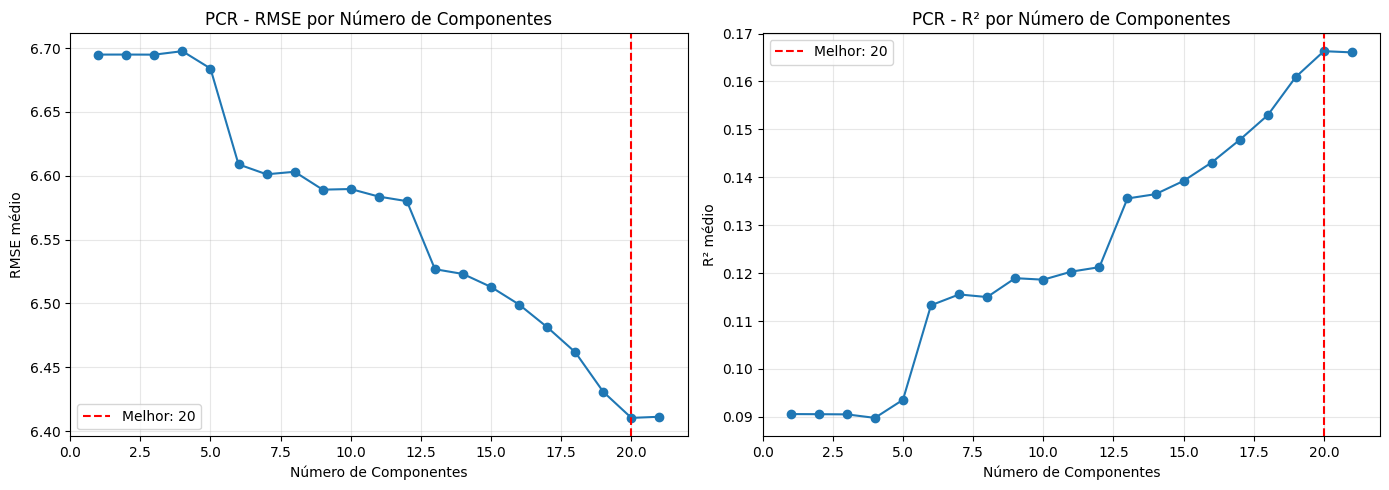
\includegraphics[width=0.7\columnwidth]{Figures/BMI.png}
    \caption{histograma do preditor BMI, com e sem classificação.}
    \label{fig:BMI}
\end{figure}


\section{Metodologia}

\subsection{Tratamento dos dados}
Inicialmente, se faz necessário fazer um pré-processamento do dataset com a finalidade de ajustar possíveis problemas associados à modelagem da regressão para uma predição mais acurada. Esse processo é dividido nos seguintes pontos: ajustar preditores com assimetria e, possivelmente, lidar com \textit{outliers}.

O dataset em questão possui apenas 3 variáveis quantitativas, duas delas sendo os preditores 'PhysHlth' e 'MentHlth' e a última sendo a saída 'BMI'. Logo, a análise de assimetria é focada nessas três colunas.

É possível perceber na <Figura tal> que todas as três variáveis possuem assimetria positiva significativa, o que justifica a aplicação de transformações de assimetria para estabilizar a variância desses preditores. Não faremos transformação apenas na saída ('BMI'). Para fazermos essa transformação, usaremos o método de Yeo-Johnson, que é dado por:
$$a$$  

Em que \lambda é o parâmetro que melhor diminui a assimetria da coluna 

Foi escolhido esse método por ser um método robusto que consegue lidar com valores negativos e nulos, possibilitando o uso garantido em todo o conjunto.

A última etapa antes de criarmos o modelo está na separação dos conjuntos de treino e de teste do projeto. Isso foi feito usando uma proporção de 75\% dos dados para treino e 25\% dos dados para teste. Em seguida, é aplicado as transformações de Yeo-Johnson no conjunto de treino e é utilizado

\subsection{Modelo OLS}



\subsection{Modelo penalizado}

Então, com o objetivo de analisar o erro dependendo da Variância e do vies, foi feito o modelo OLS adicionado de a penalização Ridge.

A ideia central é: o erro é medido como uma soma entra um erro irredutivel aleatório e  um erro redutivel, composto do viés e da variancia:

\begin{equation}
\mathbb{E}\left[(y - \hat{f}(x))^2\right] = \text{Bias}\left[\hat{f}(x)\right]^2 + \text{Var}\left[\hat{f}(x)\right] + \sigma^2
\end{equation}

Entretanto, o viés, ou Bias, é inversamente proporcional a variância, logo, para se ter o menor erro possivel, é necessário achar um ponto em que essa soma de o minimo o possível, conforme o grafico da figura \ref{fig:trade_off} 

\begin{figure}[h]
    \centering
    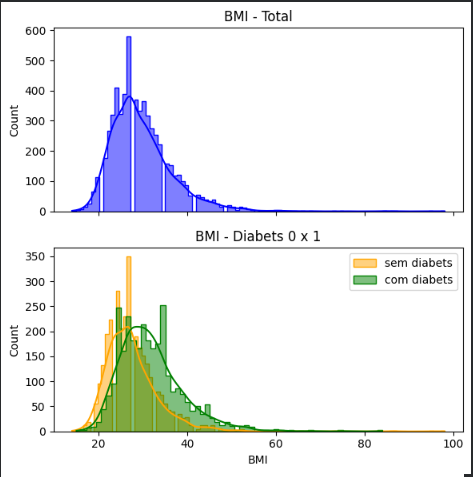
\includegraphics[width=0.7\columnwidth]{Figures/bieas_variancia.png}
    \caption{trade off entre bies e variancia}
    \label{fig:trade_off}
\end{figure}

Para tanto, adicionamos uma penalização na formula do OLS, responsável por diminuir a variancia conforme o quão grande for o lambda:

\begin{equation}
\hat{\beta} = \arg\min_{\beta} \left\{ \sum_{i=1}^{n} (y_i - \hat{y}_i)^2 + \lambda \sum_{j=1}^{p} \beta_j^2 \right\}
\end{equation}
Onde beta são os parametros do meu modelo linear

Em python, esse processo foi feito de forma matricial, definindo alguns lambdas e calculando:

\begin{equation}
\hat{\beta} = (X^T X + \lambda I)^{-1} X^T y
\end{equation}

então, para validação, foram calculados à mão para cada lambda, o RMSE e o R² feito na validação cruzada e o RMSE e o R² com os dados de teste. Também, foram comparados com funções nativas do python para verificar a corretude do algoritimo. 

Para os 10 lambdas testados, foi então montada a seguuinte tabela: tabela \ref{table:ridge}. A comparação entre os os parametros feitos a mão e utilizando funções prontas confirma a veracidade do modelo criado, pois a diferença é pequena para o cas estudado.

\begin{figure*}[!t]
    \centering
    % 1. FIGURA DE CIMA (Tela toda)
    \includegraphics[width=0.8\textwidth]{Figures/tabela_penalizada.png}
    \caption{Tabela de comparação do modelo Ridge para diferentes lambdas}
    \label{table:ridge} 
\end{figure*}  

Na seção \ref{section:result_penalizado}, está a interpretação desta tabela com alguns regursis para compreenção.

\FloatBarrier


\subsection{PCR}

A Regressão por Componentes Principais (PCR) combina a Análise de Componentes Principais (PCA) com a regressão linear, buscando reduzir a dimensionalidade dos dados e evitar problemas de multicolinearidade entre os preditores.

Após o pré-processamento dos dados, os preditores foram padronizados e submetidos ao PCA, responsável por transformá-los em componentes principais ortogonais, ordenados conforme a variância explicada. Esses componentes foram utilizados como variáveis independentes para o treinamento de um modelo de regressão linear, cuja variável resposta corresponde ao Índice de Massa Corporal (BMI).

O modelo pode ser representado pela equação:

\begin{equation}
    \hat{y} = \beta_0 + \sum_{j=1}^{k} \beta_j z_j
\end{equation}

onde $z_j$ representa o j-ésimo componente principal, $\beta_j$ corresponde ao coeficiente associado e $k$ representa a quantidade de componentes selecionados.

Para determinar o número ideal de componentes, foi realizada uma validação cruzada K-fold com 10 partições, avaliando diferentes quantidades de componentes por meio das métricas RMSE e $R^2$.

A configuração com menor RMSE médio foi selecionada para o treinamento final, utilizando todo o conjunto de treinamento. Posteriormente, o modelo foi avaliado no conjunto de teste, permitindo comparar seu desempenho com os demais métodos de regressão.

Conforme apresentado na Figura \ref{fig:pcr_graph},
a validação cruzada permitiu analisar a variação
do RMSE e do $R^2$ em função do número de componentes principais.

\subsection{Rede Neural}
O modelo de rede neural foi desenvolvido utilizando a linguagem Python e a biblioteca \texttt{sklearn.neural\_network}, por meio do algoritmo Multi-Layer Perceptron (MLP). Para o treinamento, foi utilizado o algoritmo de otimização Adam (Adaptive Moment Estimation), com parâmetro de aleatoriedade definido como 42, função de ativação ReLU (Rectified Linear Unit) nas camadas ocultas e limite máximo de 10.000 iterações.

Com o objetivo de avaliar a influência da arquitetura da rede neural no desempenho da regressão, foram testadas diferentes configurações de camadas ocultas e quantidade de neurônios. As arquiteturas avaliadas foram: uma camada oculta com 3, 6, 12, 32, 64 e 128 neurônios, além de configurações com duas camadas ocultas de 64 e 32 neurônios e três camadas ocultas de 128, 64 e 32 neurônios, respectivamente. Os resultados obtidos para cada configuração são apresentados na seção de resultados e discussão.

O MLP é uma arquitetura de rede neural composta por camadas de neurônios interconectados, nas quais os valores de entrada são processados por meio de pesos, vieses e funções de ativação. A utilização de camadas ocultas com a função de ativação ReLU permite que a rede aprenda relações não lineares entre as variáveis preditoras e a variável resposta, o Índice de Massa Corporal (IMC). Dessa forma, o modelo possui capacidade de representar relações mais complexas do que aquelas capturadas por modelos de regressão linear.

O algoritmo Adam foi empregado para otimizar os parâmetros da rede, realizando atualizações dos pesos e vieses durante o treinamento com base no gradiente da função de perda. O processo de aprendizagem ocorre iterativamente, buscando minimizar o erro entre os valores de IMC previstos pelo modelo e os valores observados no conjunto de treinamento. O encerramento do treinamento ocorre de acordo com os critérios de convergência estabelecidos pelo algoritmo ou com o atingimento do limite máximo de iterações.

\section{Resultados}

\subsection{Modelo OLS}



\subsection{Modelo penalizado}
\label{section:result_penalizado}

Como resultado do modelo Ridge, a figurar \ref{fig:parametros_ridge} demonstra o comportamento dos parametros de validação a cada lambda.

\begin{figure*}[!t]
    \centering
    % 1. FIGURA DE CIMA (Tela toda)
    \includegraphics[width=0.8\textwidth]{Figures/metricas_penalizado.pdf}
    \caption{grafico de comparação do R² e do RMSE para cada lambda}
    \label{fig:parametros_ridge}
\end{figure*}  

Segundo o grafico, quanto menor a penalisação, menor o erro. Isso revela, que o modelo OLS já estava no ponto ótimo entre vies e variância sem a penalisação, ou seja, quando lambda é igual a 0. Nota-se ainda que a que se aumenta o vies, o erro RMSE, e o R² tende a zero. Isso indica que o modelo esta se aproximando de um modelo que somente calcula a média, ou seja, quando R² = 0 e o RMSE tende ao desvio padrão, no caso 0,7.

Assim, em suma, o lambda ideal é proximo de 0, o que faz o RMSE ficar com o valor de 6,1946 e o R² ficar 0,2240; sendo assim, a uma regressão linear simples.

\subsection{PCR}


A partir da validação cruzada com 10 partições, foram selecionados 20 componentes principais, correspondentes à configuração que apresentou o menor RMSE médio. Durante a validação cruzada, o modelo obteve RMSE de 6,4104 e coeficiente de determinação ($R^2$) de 0,1663.

Após a seleção dos componentes, o modelo PCR foi treinado utilizando todo o conjunto de treinamento e avaliado no conjunto de teste, alcançando RMSE de 6,2024 e $R^2$ de 0,2258. Esses resultados indicam que o modelo conseguiu explicar aproximadamente 22,58\% da variabilidade do Índice de Massa Corporal (BMI) no conjunto de teste.

A comparação entre a implementação manual da validação cruzada e a função \texttt{cross\_validate} do Scikit-learn apresentou resultados equivalentes, confirmando a consistência dos procedimentos de avaliação utilizados.

Comparando o PCR com o modelo Ridge, que apresentou RMSE de 6,1946 e $R^2$ de 0,2240, observa-se um desempenho bastante semelhante. O PCR apresentou um erro ligeiramente superior, mas também um coeficiente de determinação um pouco maior. Essas pequenas diferenças não são suficientes para afirmar a superioridade de um dos modelos.

Dessa forma, o PCR apresentou desempenho competitivo em relação aos modelos de regressão linear avaliados, demonstrando a possibilidade de utilizar componentes principais como representação dos preditores para a previsão do BMI.

\begin{figure*}[!t]
    \centering
    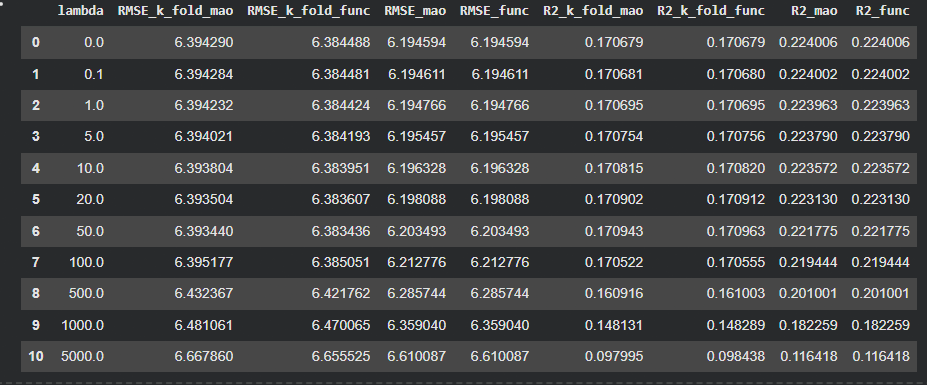
\includegraphics[width=0.8\textwidth]{Figures/pcr_graph.png}
    \caption{RMSE e R² em função do número de componentes principais.}
    \label{fig:pcr_graph}
\end{figure*}

\subsection{Rede Neural}
Os resultados obtidos para as diferentes arquiteturas de rede neural foram avaliados por meio das métricas Raiz do Erro Médio Quadrático (RMSE) e coeficiente de determinação ($R^2$), conforme apresentado na Figura \ref{fig}.

\begin{figure}[!h]
\centering
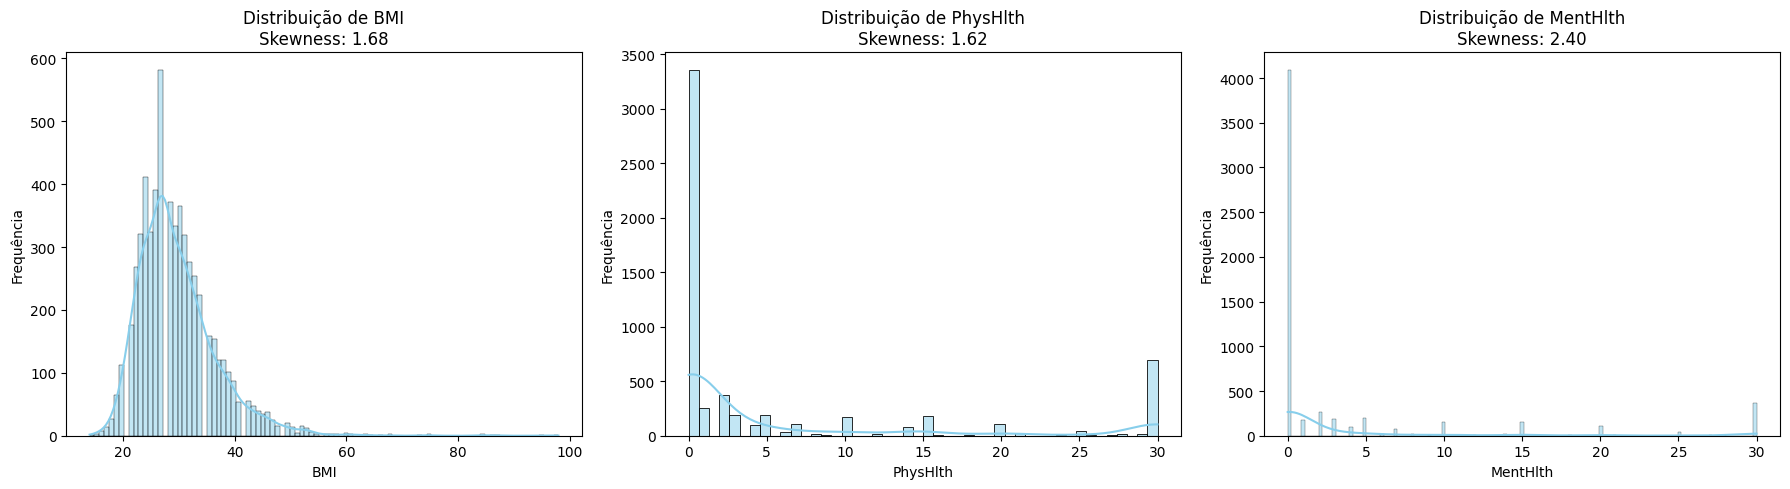
\includegraphics[width=0.4\textwidth]{Figures/resultados_rede_neural.png}
\caption{Resultados das arquiteturas de rede neural avaliadas.}
\label{fig}
\end{figure}

O modelo com uma camada oculta composta por 6 neurônios apresentou o melhor desempenho entre as arquiteturas testadas, alcançando um RMSE de 6,1480 e um coeficiente de determinação ($R^2$) de 0,2353. Esse resultado indica que o modelo explica aproximadamente 23,53\% da variabilidade observada nos valores do Índice de Massa Corporal (IMC), apresentando um erro de previsão de aproximadamente 6,15 unidades de IMC. Durante o treinamento, a arquitetura apresentou uma função de perda (Loss) de 19,39 e convergiu após 890 iterações.

A arquitetura com 6 neurônios apresentou um equilíbrio favorável entre complexidade e desempenho preditivo, quando comparada às demais configurações avaliadas. Esse comportamento pode estar relacionado ao trade-off entre viés e variância, uma vez que arquiteturas muito simples podem não capturar adequadamente as relações presentes nos dados, enquanto arquiteturas mais complexas podem apresentar maior dificuldade de generalização. Entretanto, os resultados obtidos não permitem afirmar diretamente que o modelo se encontra no ponto ótimo desse equilíbrio.

Ao comparar os resultados da rede neural com os do modelo de regressão linear desenvolvido anteriormente, observa-se que a arquitetura com 6 neurônios apresentou desempenho superior, considerando o maior valor de $R^2$ e o menor RMSE. Essa melhoria pode indicar a existência de relações não lineares entre as variáveis preditoras e o IMC, potencialmente capturadas pela capacidade de aprendizado da rede neural.

Entretanto, o valor de $R^2$ ainda relativamente baixo demonstra que uma parcela significativa da variabilidade do IMC não é explicada pelo modelo. Dessa forma, embora a rede neural tenha apresentado resultados mais satisfatórios que o modelo linear, seu poder explicativo permanece limitado. Isso pode estar relacionado à complexidade da relação entre os preditores e a variável resposta, bem como à influência de fatores não contemplados no conjunto de dados.
\begin{thebibliography}{99}

\end{thebibliography}

\vspace{12pt}

\end{document}